% CooK -- End-Semester Evaluation Report
% Same structure as the mid-semester report (title block, team and guide
% tables, numbered sections, running header, numbered references).
% Build: pdflatex (twice, for the table of contents) or upload to Overleaf.
% Figures are drawn here with TikZ/pgfplots; no image files are needed.

\documentclass[11pt,a4paper]{article}
\usepackage[margin=1in]{geometry}
\usepackage[T1]{fontenc}
\usepackage[utf8]{inputenc}
\usepackage{lmodern}
\usepackage{microtype}
\usepackage{array,booktabs,tabularx}
\usepackage{enumitem}
\usepackage{fancyhdr}
\usepackage{xcolor}
\usepackage{tikz}
\usetikzlibrary{arrows.meta,positioning}
\usepackage{pgfplots}
\pgfplotsset{compat=1.16}
\usepackage[hidelinks]{hyperref}

\pagestyle{fancy}
\fancyhf{}
\fancyhead[L]{CooK --- Endsem Evaluation Report}
\fancyfoot[C]{\thepage}
\setlength{\headheight}{14pt}
\setlength{\parskip}{6pt}
\setlength{\parindent}{0pt}
\setlist{itemsep=2pt,topsep=4pt}
\newcommand{\code}[1]{\texttt{\detokenize{#1}}}
\newcolumntype{Y}{>{\raggedright\arraybackslash}X}
\renewcommand{\arraystretch}{1.2}

\begin{document}

% ------------------------------------------------------------------ title
\begin{titlepage}
\centering
{\large National Institute of Technology Karnataka, Surathkal\par}
{\large Department of Electronics and Communication Engineering\par}
\vspace{2.5cm}
{\Huge\bfseries CooK\par}
\vspace{0.3cm}
{\Large Cluster of On-chip Konnectivity\par}
\vspace{0.6cm}
{\large A Mesh-Topology Network-on-Chip for Multi-Core RISC-V Interconnect\par}
\vspace{1.5cm}
{\Large\bfseries END-SEMESTER EVALUATION REPORT\par}
\vspace{0.4cm}
{[Course Name / Code]\par}
\vspace{1.5cm}
\begin{tabular}{|l|l|l|}
\hline
\textbf{Role} & \textbf{Name} & \textbf{Roll Number} \\ \hline
Team Member 1 & [Name] & [Roll No.] \\ \hline
Team Member 2 & [Name] & [Roll No.] \\ \hline
Team Member 3 & [Name] & [Roll No.] \\ \hline
Team Member 4 & [Name] & [Roll No.] \\ \hline
\end{tabular}

\vspace{1cm}
\begin{tabular}{|l|l|}
\hline
Guide / Instructor & [Guide Name] \\ \hline
Submission Date & [DD / MM / YYYY] \\ \hline
\end{tabular}
\vfill
\end{titlepage}

\tableofcontents
\newpage

% ------------------------------------------------------------------ 1
\section{Abstract}

CooK (Cluster of On-chip Konnectivity) is a Network-on-Chip (NoC) for a small
multi-core embedded system: a $2\times2$ mesh that connects three PicoRV32
RISC-V cores and a gateway to DDR2 memory through a Xilinx AXI DMA, targeted at
a Digilent Nexys4 DDR board. At the mid-semester milestone a single router and
a two-router link existed in simulation. This report covers the complete
system built since then: the network interface, a mesh generated from two size
parameters, the DMA/DDR gateway with its AXI bridges, and a start-up Built-In
Self Test (BIST) that tests every link and every router, shares a list of what
is dead, and routes around it. The project's own contribution is that the
self-test result is used by hardware to decide which tiles may take part in
DMA data movement.

To measure what the mesh buys, a single-bus baseline was built with the same
cores, network interfaces and software, so that only the interconnect differs.
In simulation, any single link fault leaves all three cores usable on the NoC
and none on the bus; three simultaneous traffic flows on separate paths finish
in 1,807 clock cycles on the NoC against 2,697 on the bus; and with nine nodes
sending random traffic the NoC needs 13,513 cycles where the bus needs 27,398.
With slow cores making one access at a time the bus is about 10\% faster. The cores were checked with
riscv-tests (41 of 42) and riscv-arch-test against the Spike reference model
(38 of 39) on both systems, and a three-core cryptography demonstration
(AES-128, a hash-based signature, key generation and arbitration) runs on
both. A first board session passed for the design as it stood on 7 November;
the features added after that date pass in simulation and await a new
bitstream.

% ------------------------------------------------------------------ 2
\section{Problem Statement}

A shared bus is the usual way to connect a few processors and a memory on one
chip, and it has two weaknesses that grow with the number of cores.

\begin{itemize}
\item \textbf{One channel.} Every transfer waits its turn, so transfers that
have nothing to do with each other still slow each other down.
\item \textbf{One point of failure.} A single fault on the bus stops every
core. The system cannot tell which fault it was and has no other path to keep
working on.
\end{itemize}

A Network-on-Chip answers the first weakness with several links that carry
traffic at once. It can answer the second only if the network knows which of
its own parts are healthy and acts on that knowledge. An earlier NITK
thesis~[1] built a self-test that finds faulty links in a mesh, but stopped
there: the result was reported, and nothing used it.

\textbf{The problem addressed here} is therefore twofold. First, to build a
complete small multi-core system on a mesh NoC, from the router up to memory
access, without an off-the-shelf interconnect. Second, to make the network's
knowledge of its own health a live input to how data moves: to routing, and to
the admission of DMA transfers to and from memory. The work is judged against
a single-bus system built from the same parts, on three questions: how many
cores remain usable after a fault, how the two behave under simultaneous
traffic, and what the NoC costs when neither of those applies.

% ------------------------------------------------------------------ 3
\section{Objectives}

The mid-semester objectives, with their status:

\begin{tabularx}{\textwidth}{@{}Yl@{}}
\toprule
\textbf{Objective} & \textbf{Status} \\
\midrule
Five-port router for a 2-D mesh, parameterisable & Done \\
Deterministic X-Y routing with wormhole flow control & Done \\
Fair round-robin arbitration & Done \\
Directed Verilog verification, and a cocotb/pyuvm bench & Done (cocotb: two tests) \\
Mesh of routers with PicoRV32 cores through a network interface & Done \\
DMA engine and DDR memory over AXI & Done in simulation; on the board for the earlier design \\
Stretch goal: NoC BIST & Done, extended to routers and to routing around faults \\
\bottomrule
\end{tabularx}

Objectives added during the semester:
\begin{itemize}
\item Use the BIST result in hardware: route around dead links and failed
      routers, and gate DMA on tile availability.
\item Build a single-bus baseline that differs from the NoC in the
      interconnect only, and compare the two under load and under faults.
\item Run standard RISC-V test suites and benchmarks on both systems.
\item Demonstrate a real multi-core workload: three cores doing key
      generation, AES-128 and a digital signature, with private data kept in
      each core's own tile.
\end{itemize}

% ------------------------------------------------------------------ 4
\section{Literature Review}

The design draws on four strands of prior work: routing algorithms for mesh
NoCs, self-test of on-chip interconnects, AXI-based NoC architectures, and
open-source reference implementations.

\subsection{Routing Algorithms}

X-Y routing was kept over an adaptive scheme such as Odd-Even~[3] because it
is deadlock-free by construction on a mesh and simple to verify. Adaptive
schemes improve throughput under contention at the price of turn restrictions
and a larger verification effort. The one departure made this semester is a
fixed detour around links found dead at start-up (Section~6.2.4). It is
computed once, before any traffic flows, so it has none of the reconvergence
problems of adaptive routing.

\subsection{Testability and Built-In Self-Test}

Grecu et al.~[2] established self-test of NoC interconnect as a problem
distinct from testing the cores, and the survey of~[4] covers the FIFO buffers
inside routers. The NITK thesis~[1] is the closest precedent: a five-port
router, X-Y routing, and a distributed ``ping-pong'' test in which every
router checks its own links for open and stuck-at faults and reports to a
central control unit, which works out which regions of the mesh are safe.

\subsection{AXI-Based and Application-Specific NoC Architectures}

The AXI-interconnect NoC of~[6] carries AXI semantics, including bursts and
out-of-order responses, through the network. The throughput-adaptive design
of~[5] shows how far a NoC can be specialised for a workload. Both treat the
network as healthy.

\subsection{Open-Source Reference Implementations}

OpenPiton~[8] is a manycore research platform whose mesh uses separate
networks for requests and responses. tnoc~[9] provides a full AXI4 adapter
for a SystemVerilog NoC. M3-hardware~[10] organises each tile as a
communication unit beside its compute element, which is the structure CooK
also uses. panic\_with\_cocotb~[11] was the structural reference for the
cocotb bench. The link storage follows elastic-buffer flow control~[12].

% ------------------------------------------------------------------ 5
\section{Novelty: Relation to Previous Work}

\subsection{What Is the Same}

CooK deliberately rebuilds what~[1] described: the five-port router, X-Y
routing chosen for guaranteed deadlock freedom, the ping-pong link test in the
order East, South, West, North then local, a ten-bit status per router, and a
central point that collects the results. The mesh, the wormhole lock and the
elastic link buffers are standard practice~[12]. The tile structure parallels
M3-hardware~[10]. None of this is claimed as new.

\subsection{What Is Different}

\begin{tabularx}{\textwidth}{@{}YY@{}}
\toprule
\textbf{In the earlier work~[1]} & \textbf{In CooK} \\
\midrule
The test result is reported to a control unit and stops there & The result
is used by hardware: routers avoid dead links, and the gateway refuses DMA to
or from a tile that the test could not reach \\
Links are tested & Links and the inside of each router are tested (every
crossbar path, the route for each direction, one arbitration case) \\
Results are consolidated at one point & Each router also learns the full list
of dead links, exchanged over the network on links that passed, so every
router can route around a fault \\
A faulty region is to be avoided when launching work & Traffic is rerouted,
so on the $2\times2$ mesh a single link fault costs no core at all \\
Network only & A complete system: cores, network interface, memory through a
DMA, and a measured single-bus baseline built from the same parts \\
\bottomrule
\end{tabularx}

\subsection{Against Other Architectures}

The AXI-based NoC of~[6] and the adaptive design of~[5] optimise latency and
throughput on a healthy network; they do not address faults. The open
platforms reviewed~[8]--[10] provide meshes at far larger scale, with richer
protocols, but among those reviewed none feeds a self-test result into the
admission of data movement. CooK is much smaller than any of them, and its
claim is correspondingly narrow: \emph{availability measured by an on-chip
self-test is a hardware-enforced condition on DMA transfers}, together with a
like-for-like measurement of what that availability is worth against a bus.

Three smaller points are also not found in the references reviewed: the test
vectors travel as raw words through the link FIFOs, so no routed packet is
needed for the link test; a tile is declared available only by an actual
round-trip read with a self-checking word, so a fault can never produce a
false ``healthy''; and the same network interface, software and gateway run on
both the mesh and the bus, which isolates the interconnect in every
comparison.

% ------------------------------------------------------------------ 6
\section{Proposed Methodology and System Architecture}

\subsection{Methodology}

\begin{enumerate}
\item \textbf{Build from the bottom up and verify each layer} before the next
depends on it: link buffer, router, network interface, mesh, gateway, board.
\item \textbf{Keep one source of truth for sizes.} Mesh dimensions, flit
layout and address widths are defined once; the mesh is generated, not wired
by hand. A $3\times3$ mesh runs the same software.
\item \textbf{Inject faults deliberately,} at build time and while running,
and require that no fault makes the system hang.
\item \textbf{Build the alternative.} A single-bus system with the same
cores, network interfaces and software, so that any measured difference is
the interconnect.
\item \textbf{Check against independent references:} the Spike simulator for
the processors, OpenSSL for the cipher, and deliberate breaking of the design
to confirm that the tests can fail.
\end{enumerate}

\subsection{Design}

\subsubsection{Overall Architecture}

Figure~\ref{fig:arch} shows the system. Each tile owns a window of the address
space; the upper address bits name the tile. A core is unaware of the network:
it reads and writes addresses, and its network interface (NI) turns an access
to another tile's window into a packet. Reads wait for a response; writes are
posted. Each core tile has its own block RAM, so there are no caches and no
coherence problem.

\begin{figure}[h]
\centering
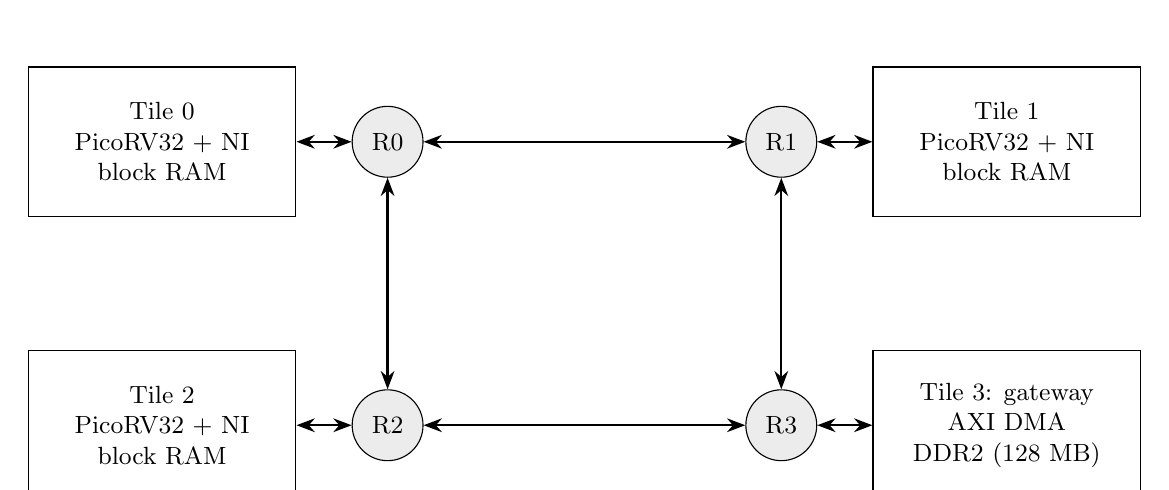
\begin{tikzpicture}[
  tile/.style={draw, minimum width=3.4cm, minimum height=1.9cm, align=center, font=\small},
  rt/.style={draw, circle, minimum size=0.9cm, font=\small, fill=gray!15},
  lk/.style={{Stealth}-{Stealth}, thick}]
\node[rt] (r0) at (0,0) {R0};
\node[rt] (r1) at (5,0) {R1};
\node[rt] (r2) at (0,-3.6) {R2};
\node[rt] (r3) at (5,-3.6) {R3};
\draw[lk] (r0) -- (r1);
\draw[lk] (r2) -- (r3);
\draw[lk] (r0) -- (r2);
\draw[lk] (r1) -- (r3);
\node[tile, left=0.7cm of r0]  (t0) {Tile 0\\PicoRV32 + NI\\block RAM};
\node[tile, right=0.7cm of r1] (t1) {Tile 1\\PicoRV32 + NI\\block RAM};
\node[tile, left=0.7cm of r2]  (t2) {Tile 2\\PicoRV32 + NI\\block RAM};
\node[tile, right=0.7cm of r3] (t3) {Tile 3: gateway\\AXI DMA\\DDR2 (128 MB)};
\draw[lk] (t0) -- (r0);
\draw[lk] (t1) -- (r1);
\draw[lk] (t2) -- (r2);
\draw[lk] (t3) -- (r3);
\end{tikzpicture}
\caption{The CooK system. Four routers in a $2\times2$ mesh; every link is two
one-way FIFOs. A BIST node (not drawn) sits between each router and its links.}
\label{fig:arch}
\end{figure}

\subsubsection{Router and Links}

\begin{tabularx}{\textwidth}{@{}lY@{}}
\toprule
\textbf{Block} & \textbf{Function} \\
\midrule
Packet & Two flits, HEAD then TAIL, 44 bits each on the default mesh: 32 data
bits, absolute destination, source tile, flit type, a poison bit and five
parity bits. Routers forward flits unchanged, so the sender's parity is
checked end to end. \\
Route computation & X-Y on the absolute destination. With a dead link on the
$2\times2$ mesh, the way round the ring that crosses no dead link. \\
Route holding & An output is locked to one packet from its HEAD to its TAIL,
so packets cannot interleave. At mid-semester this lock did not exist; adding
it fixed a reproduced interleaving bug. \\
Arbitration & Round robin per output; the pointer moves only when a new packet
is granted. \\
Link buffers & A FIFO of six flits on every link, with a registered ready
signal. The router itself stores nothing (elastic-buffer flow control~[12]).
A HEAD is admitted only when the next FIFO has room for the whole packet. \\
Fault handling & Parity failure, an orphan flit, or a HEAD for a missing or
dead port is dropped; a packet cut short is closed with a poison TAIL; a
watchdog per output marks a stalled output dead. \\
\bottomrule
\end{tabularx}

Whole-packet admission has a useful consequence: in a healthy network a locked
output never sees its downstream FIFO fill, so a stalled locked output is a
fault and not congestion. The watchdog relies on that distinction.

\subsubsection{Network Interface}

The NI serves a core's local accesses from the tile's block RAM and registers
without touching the network. For a remote read it sends a request and waits;
if no response arrives it retries with a new tag, and after three attempts
returns a poison value and sets a flag, so a core never hangs. It answers
other tiles' reads in hardware, whether or not its own core is running, which
is what lets the gateway judge a tile's availability. Another tile may write
only the tile's mailbox window, and with an option enabled may read only that
window and the status registers.

\subsubsection{BIST Module}

A BIST node sits between each router and its links. After every full reset,
and before any core runs, it takes over the router's ports and runs a fixed
schedule. All nodes leave reset on the same clock edge and stay in step by
counting cycles. The whole sequence takes 545 cycles, about 11~$\mu$s at
50~MHz.

\begin{enumerate}
\item \textbf{Link test.} In turn for each direction, a router sends six test
words alternating all-zeros and all-ones; the neighbour checks them and
returns one acknowledgement word. Each router records ten bits: an inbound
and an outbound result for each of its five ports. Every bit starts as
``failed'' and only a passed test sets it.
\item \textbf{Router self-test.} For every input port and every other output
port, a test packet addressed to leave by that output is applied to that
input. Exactly its two flits must appear on that output, in order and
unchanged, and nothing may appear elsewhere. Two inputs are then driven at
once towards the local output to check that the packets come out whole.
\item \textbf{Dead-link list.} Routers exchange a mask with one bit per
physical link, over links that passed only, until all hold the same mask. A
router that failed its self-test reports all of its own links.
\item \textbf{Use.} Both ends stop using a dead link, and routes go the other
way round the ring. Removing a link from a ring leaves a line, which has no
cycle, so the detour cannot create a deadlock.
\item \textbf{Availability.} The gateway reads each tile's status over the
network. A tile is available only if that read returns, with a self-checking
(complemented) word. The cores are released after this.
\end{enumerate}

On the board, the results appear as error codes: \code{E} for a failed link
and \code{F} for a failed router, each with the tile number and the failed
ports.

\subsubsection{DDR and DMA Gateway}

Tile~3 has no core. Its gateway connects the network to the board's 128~MB
DDR2 memory through the Xilinx AXI DMA~[19] and memory controller~[20]. A core
moves a block between its own RAM and the DDR in three steps: claim the DMA
lock, program the transfer, wait for completion. The gateway enforces, in
hardware:
\begin{itemize}
\item a lock on the DMA, claimed by a read (safe if the NI retries), handed on
round robin, with a lease so that a silent owner loses it;
\item checks at the write that starts a transfer: only permitted registers,
word alignment, the owner's own tile only, length within the tile, and the
tile's availability from BIST;
\item zones in the DDR: three 40~MB zones, one per core, and two 4~MB shared
windows;
\item a reason code for every refused request.
\end{itemize}

The availability check is the link this project set out to make: a tile that
the self-test could not reach cannot take part in a DMA transfer.

\subsubsection{AXI Bridges}

AXI appears only where the Xilinx IP requires it. The cores use PicoRV32's
native interface, one request at a time, which already has the shape of a
packet stream; wrapping it in AXI's five channels and unwrapping it again
would add logic and no function.

\begin{tabularx}{\textwidth}{@{}lY@{}}
\toprule
\textbf{Bridge} & \textbf{What it converts} \\
\midrule
Packets to AXI4-Lite & A core's read or write of the gateway's register
window becomes an AXI4-Lite transaction on the DMA's control port. An AXI
error response is returned to the core as a poison value. \\
AXI4-Stream to packets & Each word the DMA streams out of the DDR becomes a
posted write packet into the destination tile's RAM, with the address
advancing. \\
Packets to AXI4-Stream & To move RAM to DDR, the gateway reads the source
tile word by word over the network and feeds the DMA's input stream. \\
AXI4 to the memory controller & The DMA's memory-mapped ports reach the MIG
through a SmartConnect, which also crosses from the 50~MHz system clock to
the controller's own clock. This part is Xilinx IP, assembled by a script. \\
Packets to AXI4 (baseline) & In the single-bus system a memory node turns a
packet into a single-beat AXI4 read or write towards the same controller. \\
\bottomrule
\end{tabularx}

\subsubsection{Isolation and Recovery}

Any tile can read whether another tile's core has trapped and restart it
through a register in that tile's NI; on a restart the start-up code restores
the program's initialised data. Mutual exclusion on shared memory words is
left to firmware, a deliberate decision discussed in Section~8.

\subsubsection{Single-Bus Baseline}

For comparison, a second system replaces the mesh with one shared channel
that carries the same packets: a transmit queue per node, a round-robin
arbiter that grants the channel for a whole packet, and a watchdog. The core
tiles use the NoC's NI, block RAM and software unchanged, and for the fabric
benchmark the same DMA gateway is attached. It is not a textbook AXI bus; it
is the closest single-channel equivalent of the NoC, so that any measured
difference is due to the interconnect. It has its own board top and Vivado
project scripts.

% ------------------------------------------------------------------ 7
\section{Work Completed to Date}

\subsection{Summary}

\begin{tabularx}{\textwidth}{@{}lY@{}}
\toprule
\textbf{Component} & \textbf{What was built since mid-semester} \\
\midrule
\code{noc_router.v} & Rewritten: output lock, whole-packet admission, parity,
poison TAILs, watchdog, routing around dead links \\
\code{link_buffer.v} & From a single slot to a FIFO with registered ready
(the single-slot version formed a combinational loop round the mesh) \\
\code{ni.v} & Network interface: local RAM and registers, remote read and
posted write, timeout and retry with tags, response queue, write and read
windows, core restart \\
\code{noc_mesh.v}, \code{mesh_top.v} & Mesh generated from two size
parameters; $3\times3$ runs the same software \\
\code{bist_node.v} & Link test, router self-test, dead-link exchange \\
\code{gw_ni.v} & DMA gateway with lock, checks, zones and BIST collection \\
Board top & Clocking, reset, status panel with error codes, fault-injection
switches, optional serial port \\
\code{single_bus/} & Shared bus, memory node, system and board tops \\
\code{benchmarks/} & C runtime and linker script; runners for the test
suites, benchmarks and the fabric comparison \\
\code{encryption_code/}, \code{demo_tests/} & Cryptography demonstration,
laptop link, board demonstrations \\
\bottomrule
\end{tabularx}

All results below are from simulation with Icarus Verilog unless a line says
otherwise.

\subsection{Tests: Simulation and Functional Verification}

\subsubsection{Why These Tests}

Each layer is tested alone before the next is built on it, because a fault in
a lower layer shows up above as something else entirely: the packet
interleaving bug in the router first appeared as a hung core. Every testbench
checks its own results, and the regression fails if any check fails. Three
practices go beyond directed tests:
\begin{itemize}
\item \textbf{Fault injection,} because the project's claims are about
faults. A link can be made silent or made to flip a bit, and a router can be
made to corrupt its output, at build time or while running.
\item \textbf{Mutation checks,} because a test that cannot fail proves
nothing. The design is deliberately broken (routing reversed, the output lock
removed, the detour disabled) to confirm that the tests go red.
\item \textbf{Randomised traffic with a scoreboard,} because directed tests
only cover the cases their author thought of, and deadlock is a property of
unplanned interleavings.
\end{itemize}

\subsubsection{Directed Tests}

\begin{tabularx}{\textwidth}{@{}Ylr@{}}
\toprule
\textbf{Suite} & \textbf{Scope} & \textbf{Checks} \\
\midrule
Address decoder, link buffer & units & 17, 229 \\
Router (directed), router (cocotb) & unit & 159, 2 tests \\
Network interface & unit & 66 \\
BIST: six meshes, each with a different fault & fabric & 18 \\
Mesh with real cores: healthy, faults, $3\times3$, all-to-all & system & 75 \\
Gateway with DMA model, healthy and faulted & system & 67 \\
Status panel, board top & board logic & 61, 20 \\
Single-bus baseline, all suites & baseline & 10 suite runs \\
\bottomrule
\end{tabularx}

All pass. Synthesis checks with Yosys report no latches and no combinational
loops in either fabric.

\subsubsection{Availability Under Faults}

This test answers the first question of the problem statement. Every directed
link was faulted in turn, in both modes, on the system with the gateway and
three cores running a program that tests every other tile.

\begin{tabularx}{\textwidth}{@{}Ycc@{}}
\toprule
\textbf{Fault} & \textbf{NoC: cores usable} & \textbf{Bus: cores usable} \\
\midrule
Any single link, silent or bit-flip (16 cases) & 3 of 3 & 0 of 3 \\
One router broken inside & 2 of 3 & --- \\
Both links of one tile & 2 of 3 & --- \\
Two opposite links (mesh split) & 1 of 3 & --- \\
\bottomrule
\end{tabularx}

The bus figure is for a stuck arbiter or a flipped data wire: one shared
resource and no other path. No core hangs in any case; a core that cannot
reach its target receives a poison value and an error flag. A separate test
breaks a link \emph{after} the self-test has finished: nothing reroutes, the
affected read times out and returns the poison value, and the system carries
on.

\subsubsection{Randomised Traffic}

Every node issues 1,000 random accesses to random other nodes, all at once,
with random pauses. A scoreboard records what each memory word must hold; each
read is checked against it, and at the end every word is compared. The test
passed on the $2\times2$ mesh (three seeds), the $3\times3$ mesh, the
$2\times2$ mesh with a dead link, and the bus with four and nine nodes, about
19,000 checked reads in all: no access hung and no packet was lost, duplicated
or misdelivered.

This is evidence from random testing and not a proof. It covers the operating
condition the design assumes, at most one read outstanding per node; the
structural argument for that condition is in Section~8.

\subsection{Benchmarks}

\subsubsection{Why Standard RISC-V Suites}

Two suites maintained under RISC-V International were run on both systems,
for a specific reason. Every other result in this report assumes the cores
compute correctly. If a core were subtly wrong, a failure in a system test
could not be attributed to the interconnect. The standard suites settle that
independently of anything written for this project:
\begin{itemize}
\item \textbf{riscv-tests}~[13] exercises each base instruction with
self-checking cases.
\item \textbf{riscv-arch-test}~[14] is the architectural compliance suite;
each test leaves a signature in memory, which is compared with the signature
produced by the Spike reference simulator~[15] for the same program.
\item \textbf{Dhrystone}~[16] and \textbf{CoreMark}~[17] are the two
benchmarks by which small cores are commonly placed, so they locate this
system on a familiar scale.
\end{itemize}
Adapting them required a C runtime, a linker script that keeps a program
clear of the tile's mailbox, and a reporting convention, since a tile has no
console, no timer and no control registers.

\subsubsection{Results}

\begin{tabularx}{\textwidth}{@{}Yll@{}}
\toprule
\textbf{Suite} & \textbf{Result (both systems)} & \textbf{Note} \\
\midrule
riscv-tests rv32ui~[13] & 41 of 42 & \code{ma_data} needs misaligned access \\
riscv-arch-test RV32I~[14] against Spike~[15] & 38 of 39 & \code{jal-01} exceeds the largest tile \\
Dhrystone 2.1~[16] & 7.23 DMIPS at 50~MHz & 0.145 DMIPS/MHz \\
CoreMark~[17] & 11.30 at 50~MHz & 0.226 CoreMark/MHz \\
\bottomrule
\end{tabularx}

The cores are RV32I with no multiplier and no barrel shifter, which accounts
for the low scores. One line of PicoRV32 was changed so that \code{fence.i}
is accepted as a no-operation, which is correct for a core with no
instruction cache.

\textbf{These results are identical on the NoC and on the bus, and that is
expected.} The programs run inside one tile and never use the interconnect.
They establish that the cores are correct in both systems; they cannot compare
the systems. That comparison needs traffic, which is the next benchmark.

\subsubsection{NoC Against Bus Under Load}

In the fabric benchmark the cores are replaced by drivers that issue accesses
back to back, because a PicoRV32 issues so few accesses that either fabric
sits mostly idle. The endpoints, including the DMA gateway, are identical on
both fabrics. Three flows of 448 words are run alone and then together
(Figure~\ref{fig:fabric}): a DMA stream from DDR into tile~0, tile~1 writing
to tile~2, and tile~2 writing to tile~1. On the mesh the three share no link.

\begin{figure}[h]
\centering
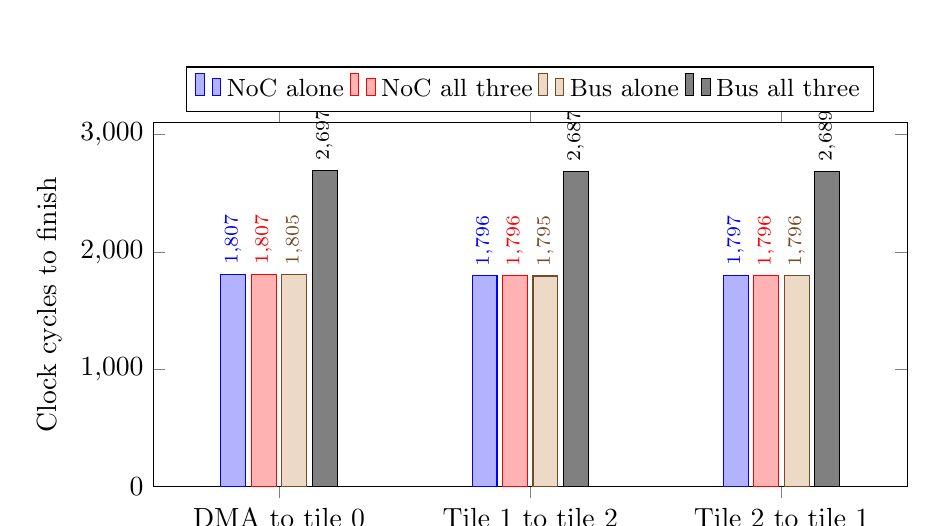
\begin{tikzpicture}
\begin{axis}[ybar, bar width=9pt, width=0.92\textwidth, height=6.2cm,
  ylabel={Clock cycles to finish}, ymin=0, ymax=3100,
  symbolic x coords={DMA to tile 0, Tile 1 to tile 2, Tile 2 to tile 1},
  xtick=data, enlarge x limits=0.25,
  legend style={at={(0.5,1.03)}, anchor=south, legend columns=4, font=\small},
  nodes near coords, every node near coord/.append style={font=\scriptsize, rotate=90, anchor=west}]
\addplot coordinates {(DMA to tile 0,1807) (Tile 1 to tile 2,1796) (Tile 2 to tile 1,1797)};
\addplot coordinates {(DMA to tile 0,1807) (Tile 1 to tile 2,1796) (Tile 2 to tile 1,1796)};
\addplot coordinates {(DMA to tile 0,1805) (Tile 1 to tile 2,1795) (Tile 2 to tile 1,1796)};
\addplot coordinates {(DMA to tile 0,2697) (Tile 1 to tile 2,2687) (Tile 2 to tile 1,2689)};
\legend{NoC alone, NoC all three, Bus alone, Bus all three}
\end{axis}
\end{tikzpicture}
\caption{Three simultaneous flows on separate paths: the NoC is unaffected,
the bus takes 1.5 times as long.}
\label{fig:fabric}
\end{figure}

One flow at a time, the fabrics are equal: the NI, at four cycles per word, is
the limit. Together, the three flows need one and a half times what one
channel can carry. The combined work finishes in 1,807 cycles on the NoC and
2,697 on the bus.

The random-traffic test, run with identical access sequences on both fabrics,
shows how the two scale (Figure~\ref{fig:scale}).

\begin{figure}[h]
\centering
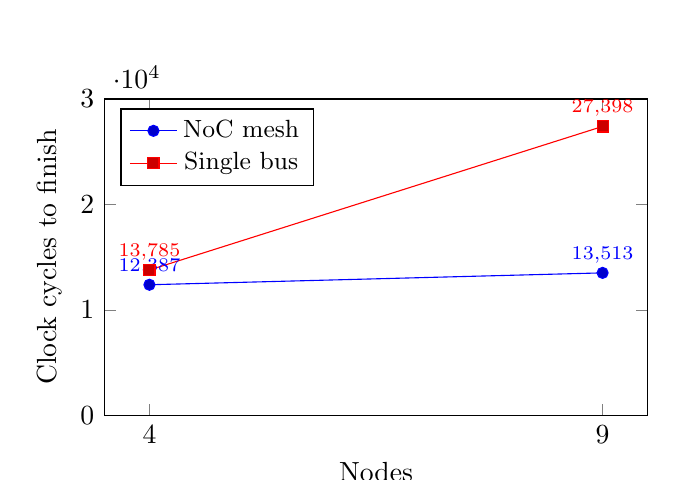
\begin{tikzpicture}
\begin{axis}[width=0.7\textwidth, height=5.6cm, xlabel={Nodes},
  ylabel={Clock cycles to finish}, xtick={4,9}, ymin=0, ymax=30000,
  legend pos=north west, legend style={font=\small},
  nodes near coords, every node near coord/.append style={font=\scriptsize}]
\addplot+[mark=*] coordinates {(4,12387) (9,13513)};
\addplot+[mark=square*] coordinates {(4,13785) (9,27398)};
\legend{NoC mesh, Single bus}
\end{axis}
\end{tikzpicture}
\caption{1,000 random accesses from every node. From four to nine nodes the
NoC's time is almost unchanged; the bus's doubles.}
\label{fig:scale}
\end{figure}

\subsubsection{The Cost: One Access at a Time}

The limits of these results should be stated with them. The gain needs traffic
that is simultaneous and on different paths. A single flow, or two flows into
the same tile, gain nothing. To measure the opposite case with real
processors, thirty-five of the riscv-tests were run with each core executing
code stored in another tile's memory, three cores at once, so that every
instruction fetch is a remote read. All pass on both systems.

\begin{tabularx}{\textwidth}{@{}Yr@{}}
\toprule
\textbf{Where the 35 tests ran} & \textbf{Total cycles} \\
\midrule
From the core's own tile & 49,249 \\
From another tile, over the NoC & 184,817 \\
From another tile, over the bus & 165,536 \\
\bottomrule
\end{tabularx}

A PicoRV32 waits for each access before issuing the next, so neither fabric is
loaded, and the bus is about 10\% faster because the mesh adds hops. This is
the price of the NoC at this scale.

\subsection{Cryptography and Demonstration Tests}

These tests show the system doing recognisable multi-core work, with real
cores and real programs, and they exercise features that the unit tests reach
only one at a time.

\subsubsection{Cryptography on Three Cores}

\begin{tabularx}{\textwidth}{@{}llY@{}}
\toprule
\textbf{Core} & \textbf{Role} & \textbf{What stays private to its tile} \\
\midrule
0 & Key generation and arbiter & the nonce and the verification state \\
1 & AES-128~[21]: encrypt, then decrypt & round keys, S-boxes, block state \\
2 & Digital signature & secret chain values, hash state \\
\bottomrule
\end{tabularx}

Core~0 derives an AES key and a signing seed with SHA-256~[22], sends core~1
a block to encrypt and core~2 a message to sign at the same time, sends the
ciphertext back to be decrypted, and verifies the signature. Jobs and results
travel only through mailboxes and carry a keyed checksum, so a message from a
core without the key is ignored. All code is C for RV32I, with no multiplier
and no floating point.

\begin{tabularx}{\textwidth}{@{}Yl@{}}
\toprule
\textbf{Check} & \textbf{Result} \\
\midrule
SHA-256 and AES-128 against the FIPS vectors, on the development machine & pass \\
Full run on the NoC and on the bus & pass, 4.52 million cycles \\
First ciphertext bytes against OpenSSL with the same key and plaintext & equal \\
Core~0 tries to read core~1's private memory (read window on) & refused \\
Core~0 sends core~1 a job with a wrong checksum & ignored \\
Changed message offered with the original signature & rejected \\
NoC with the direct link between core~0 and core~1 dead from reset & pass \\
Bus with a stuck arbiter & fails at once, reported \\
\bottomrule
\end{tabularx}

The signature is a Winternitz one-time scheme over SHA-256~[23] and not
ML-DSA. ML-DSA needs more working memory than a tile holds and is dominated
by multiplication, which these cores perform in software; a hash-based scheme
needs only the hash. The simulated run uses a reduced signature size, and the
full-size images are built for the board.

\subsubsection{Other Demonstrations}

\begin{tabularx}{\textwidth}{@{}YY@{}}
\toprule
\textbf{Demonstration and what it shows} & \textbf{Result in simulation} \\
\midrule
Parallel speed-up: the same hashing work on one core, then shared among
three & 2.89 times faster, equal digests \\
DMA with lock contention: three cores each move a block to DDR and back,
three rounds, taking turns on the lock & pass, all data equal \\
Continuous traffic with a link killed mid-run, no reset: detection without
repair & the two cores using that link report failure, the third continues \\
Restart: core~1 traps, core~0 sees it and restarts it & pass; initialised
data restored \\
Laptop link over a serial port: the laptop sends ciphertext, the board
decrypts it and shows the text; or the board encrypts and the laptop checks &
pass, equal to the laptop's AES \\
\bottomrule
\end{tabularx}

The laptop link exists to show that the computation happens on the board: the
laptop sends ciphertext only, and the plaintext appears on the board's own
display, produced by core~1 and carried across the network to core~0. Its
hardware, a serial port on core~0, is optional and is not built unless
enabled.

\subsection{Board Result}

A build with the gateway met timing at 50~MHz on the xc7a100t-1 with 1.3~ns
of slack, using 17,379 LUTs (27\%), 16,219 flip-flops and 5 block-RAM tiles.
A board session on 7 November passed the healthy test and the single-link
fault switches. That bitstream predates the router self-test, the wait for
DDR calibration, the read window, the restart register and the serial port;
those, the single-bus build, and the larger tiles used by the benchmarks and
demonstrations have not yet run on the board.

% ------------------------------------------------------------------ 8
\section{Design Choices and Known Trade-offs}

\subsection{Assumptions}

\begin{tabularx}{\textwidth}{@{}lY@{}}
\toprule
A1 & Each core has at most one remote read outstanding. \\
A2 & One clock and one reset; every node leaves reset on the same edge. \\
A3 & Faults are permanent and present at start-up. \\
A4 & Faults are in links and routers; cores, NIs, memories and the BIST logic
are taken to work. \\
A5 & Firmware cooperates: one writer per shared word, and the DMA lock is
released. \\
A6 & The mesh is $2\times2$ for routing around faults. \\
A7 & Power and the USB link are stable during a DMA transfer. \\
\bottomrule
\end{tabularx}

\subsection{Choices, Gains and Risks}

\begin{tabularx}{\textwidth}{@{}YYY@{}}
\toprule
\textbf{Choice} & \textbf{Gain} & \textbf{Risk or cost} \\
\midrule
X-Y routing, no virtual channels & Cannot deadlock by construction; small
routers & One path per pair in normal operation; depends on A1 \\
Storage on the links, whole-packet admission & A stalled output is a fault,
so a watchdog can act & FIFO memory on every link \\
BIST once after reset & A fault is found and named before any core runs &
A fault that appears later is detected but not routed around \\
Detour round the ring & A single link fault costs no core & Works on
$2\times2$ only \\
Availability by a real round-trip read & A false ``healthy'' is impossible &
The gateway is a single point of failure \\
DMA lock, lease, zones and checks in hardware & A faulty core cannot hold or
overrun the DDR & A fixed zone split \\
Native core interface, AXI only at the gateway & Small NI; no conversion to
AXI and back & Not an AXI network; no bursts, so each word is a packet \\
No atomic operation between cores in hardware & Small NI; firmware sets the
policy & Two cores can race on a shared word, silently \\
Mailbox sender check in firmware & No change to hardware & A program holding
the key can still forge; 32-bit tag \\
Write window always, read window optional & Private data stays private when
enabled & Off by default, because one test fetches code remotely \\
No caches & No coherence problem & Not a shared-memory multiprocessor in the
usual sense \\
Same NI and software on the baseline & Differences are the interconnect's &
The baseline is not a textbook bus \\
\bottomrule
\end{tabularx}

\subsection{Deadlock Freedom}

The argument is structural. X-Y routing forbids every turn from Y to X, so the
channel dependency graph has no cycle. With a dead link on the $2\times2$
mesh, no route crosses that link and no route turns back, so neither direction
round the ring can close a cycle. Requests and responses share the network;
this is safe because each node has at most one read outstanding (A1) and the
NI's response queue is sized for it. The random-traffic test supports this
under A1 and does not extend it beyond A1.

\subsection{How the System Fails}

\textbf{If firmware is wrong.} Hardware catches a write outside a mailbox, a
read of private memory when the read window is on, a DMA request for the
wrong tile, zone or length, an address that belongs to no tile, and a lock
that is never released. Hardware does not catch two cores writing the same
shared word, a program that ignores a poison value or an error flag, a stack
overrun inside a tile, or a core that restarts another without cause. The
first of these is the main risk taken: a firmware mistake on a shared word
corrupts data silently.

\textbf{If a link or router breaks while running.} Nothing reroutes, since
BIST has finished. The router's watchdog marks the output dead, reads across
it time out after three attempts and return a poison value with a flag, and
cores that do not use that path continue. A posted write lost in this way is
not reported to its sender unless firmware reads back or checks the mailbox
checksum. The system as a whole does not hang; a full reset reruns BIST,
which then finds the fault and routes around it where it can.

% ------------------------------------------------------------------ 9
\section{Limitations and Future Work}

\subsection{Known Limitations}

\begin{itemize}
\item Routing around a fault works on the $2\times2$ mesh only.
\item Deadlock freedom depends on assumption A1.
\item A fault that appears after start-up is detected but not routed around.
\item The gateway is a single point of failure for memory.
\item The router self-test does not exercise the watchdog or the drop paths.
\item The mailbox sender check is firmware, with a 32-bit tag.
\item The features added after 7 November, the single-bus Vivado project and
any build with the larger tiles used by the benchmarks have not yet run on
the board.
\end{itemize}

\subsection{Future Work}

\begin{tabularx}{\textwidth}{@{}YY@{}}
\toprule
\textbf{Topic} & \textbf{What it has to solve first} \\
\midrule
Fixing the limitations above & Separate request and response channels;
deadlock-free rerouting tables for larger meshes; re-test at run time \\
Formal verification of deadlock freedom, packet integrity, the router lock
and the gateway lock & Stating the properties and the environment assumptions \\
Caches with a coherence protocol (MESI; snooping or directory), the step to
true multiprocessing & A mesh has no shared wire to snoop, so a directory
scheme or an ordered broadcast must be chosen; ends A1 \\
Dynamic X-Y routing, and a comparison of buffers inside the router against
the present storage-free crossbar & Adaptive routing reopens deadlock and
packet ordering \\
In-order and out-of-order cores & Faster cores load the fabric; an
out-of-order core issues several accesses at once, again ending A1 \\
Extension to $3\times3$ and beyond & Rerouting beyond the ring; BIST time
grows with size \\
A second memory element & A second gateway, and lock and zone ownership
across two \\
\bottomrule
\end{tabularx}

Caches, out-of-order cores and larger meshes all remove assumption A1.
Separate request and response channels are therefore the common prerequisite,
and formal verification of the deadlock property is worth doing before any of
them. Machine-learning-based verification is noted as optional and is not
planned.

% ------------------------------------------------------------------ 10
\section{Tools and Technologies Used}

\begin{itemize}
\item Verilog (IEEE 1364) for all RTL and testbenches.
\item Icarus Verilog and GTKWave for simulation; cocotb with pyuvm for the
router bench; Yosys for synthesis checks.
\item Xilinx Vivado for synthesis and implementation on the Nexys4 DDR
(xc7a100tcsg324-1), with the AXI DMA~[19] and MIG~[20] IP.
\item PicoRV32~[7] as the core; the RISC-V GNU toolchain~[18] for assembly and C.
\item Spike~[15] as the reference model; riscv-tests~[13],
riscv-arch-test~[14], Dhrystone~[16] and CoreMark~[17] as test and benchmark
sources; Python for the runners.
\end{itemize}

% ------------------------------------------------------------------ 11
\section{Challenges Faced}

\begin{itemize}
\item \textbf{Packets interleaving on a shared output.} The router reserved
its inputs' routes but not its outputs. Reproduced in simulation and fixed
with the per-output lock.
\item \textbf{A combinational loop round the mesh.} The single-slot link
buffer chained its ready signal through every router. Replaced by a FIFO with
registered ready.
\item \textbf{A request/response deadlock} in the first NI, which refused new
input while its own response was unsent. Fixed with a response queue.
\item \textbf{Hand wiring.} All four NIs were once attached to the wrong
router port with the same tile number. The mesh is now generated.
\item \textbf{Faults that simulation could not show.} On the board the cores
started before the DDR had calibrated; the model of the memory is always
ready. Found by review, not by test.
\item \textbf{Tests that passed for the wrong reason.} A build flag silently
skipped a benchmark's result check; a regression kept driving switch values
that no longer injected a fault after three faulty board switches forced a
remapping.
\item \textbf{A new test breaking an old feature.} The router self-test ran
while a debug override had a port switched off, and cut the router out. The
override now applies only after BIST.
\item \textbf{Benchmarks that could not show the result.} Processor
benchmarks give equal numbers on both fabrics because they never leave a
tile. A separate fabric benchmark with fast drivers was needed.
\end{itemize}

% ------------------------------------------------------------------ 12
\section{Conclusion}

The system planned at mid-semester is complete in simulation and its earlier
form has run on the board: a generated mesh of routers, three PicoRV32 cores
behind network interfaces, and a gateway to DDR2 through an AXI DMA. Beyond
that plan, the network tests its own links and routers at start-up, routes
around what it finds, and uses the result to decide which tiles may move data
through the DMA, which is the link the earlier thesis~[1] left open.

Measured against a single bus built from the same parts, the NoC does not
speed up a program that stays in one tile, and for one access at a time it is
about 10\% slower than the bus. It does keep
all three cores usable after any single link fault where the bus keeps none,
it carries simultaneous transfers on separate paths without slowing them, and
its time for random traffic is almost unchanged from four nodes to nine where
the bus's doubles. These results are from simulation. The assumptions they
rest on, chiefly one outstanding read per core and faults present at
start-up, are stated with the risks they carry, and they set the order of the
future work: separate request and response channels and formal verification
first, then caches, faster cores and larger meshes.

% ------------------------------------------------------------------ refs
\section{References}

\begin{enumerate}[label={[\arabic*]}, leftmargin=2.2em]
\item Shashank V, ``Network-on-Chip Built-In Self Test for Enhancing
Availability of Multi-Processor System-on-Chip,'' B.Tech. project report,
Dept. Electron. Commun. Eng., Nat. Inst. Technol. Karnataka, Surathkal,
India, Nov. 2018.
\item C. Grecu, P. P. Pande, A. Ivanov, and R. Saleh, ``BIST for
network-on-chip interconnect infrastructures,'' in \emph{Proc. 24th IEEE VLSI
Test Symp. (VTS)}, 2006.
\item Zhang, Hou, Wang, Geng, and Wu, ``Comparison research between XY and
odd-even routing algorithm of a 2-dimension $3\times3$ mesh topology
network-on-chip,'' in \emph{Proc. WRI Global Congress on Intelligent Systems
(GCIS)}, 2009.
\item S. Ram Suja and M. Deivakani, ``Testing of FIFO buffer of NoC router
using BIST: Survey,'' \emph{Int. J. Emerging Technol. Eng. Res.}, vol. 5,
no. 1, Jan. 2017.
\item M. A. Zhiri, H. Krichene, C. Sandionigi, and S. Pillement, ``HT-NoC: A
throughput-adaptive multi-dataflow network-on-chip for AI accelerators,''
\emph{ACM Trans. Reconfigurable Technol. Syst.}, 2026,
doi: 10.1145/3808228.
\item N. Malladhi and G. V. Attimarad, ``Design and development of novel AXI
interconnect based NoC architecture for SoC with reduced latency and improved
throughput,'' \emph{Int. J. Comput. Digital Syst.}, vol. 17, no. 1, 2025.
\item C. Wolf et al., ``PicoRV32: A size-optimized RISC-V CPU,'' GitHub
repository, YosysHQ. \url{https://github.com/YosysHQ/picorv32}
\item J. Balkind et al., ``OpenPiton,'' GitHub repository, Princeton
University. \url{https://github.com/PrincetonUniversity/openpiton}
\item T. Ishitani, ``tnoc: Network-on-chip implementation written in
SystemVerilog,'' GitHub repository.
\url{https://github.com/taichi-ishitani/tnoc}
\item Barkhausen Institut, ``M3-hardware,'' GitHub repository.
\url{https://github.com/Barkhausen-Institut/M3-hardware}
\item opensmartnic, ``panic\_with\_cocotb,'' GitHub repository.
\url{https://github.com/opensmartnic/panic_with_cocotb}
\item G. Michelogiannakis, J. Balfour, and W. J. Dally, ``Elastic-buffer flow
control for on-chip networks,'' in \emph{Proc. IEEE Int. Symp.
High-Performance Computer Architecture (HPCA)}, 2009.
\item RISC-V International, ``riscv-tests,'' GitHub repository.
\url{https://github.com/riscv-software-src/riscv-tests}
\item RISC-V International, ``riscv-arch-test,'' release 3.9.1, GitHub
repository. \url{https://github.com/riscv-non-isa/riscv-arch-test}
\item RISC-V International, ``Spike RISC-V ISA simulator,'' GitHub
repository. \url{https://github.com/riscv-software-src/riscv-isa-sim}
\item R. P. Weicker, ``Dhrystone: a synthetic systems programming
benchmark,'' \emph{Commun. ACM}, vol. 27, no. 10, 1984.
\item EEMBC, ``CoreMark,'' GitHub repository.
\url{https://github.com/eembc/coremark}
\item RISC-V International, ``RISC-V GNU compiler toolchain,'' GitHub
repository. \url{https://github.com/riscv-collab/riscv-gnu-toolchain}
\item Xilinx, \emph{AXI DMA LogiCORE IP Product Guide}, PG021.
\item Xilinx, \emph{7 Series FPGAs Memory Interface Solutions User Guide},
UG586.
\item National Institute of Standards and Technology, \emph{Advanced
Encryption Standard (AES)}, FIPS 197.
\item National Institute of Standards and Technology, \emph{Secure Hash
Standard (SHS)}, FIPS 180-4.
\item R. C. Merkle, ``A certified digital signature,'' in \emph{Advances in
Cryptology --- CRYPTO '89}, 1989.
\end{enumerate}

\end{document}
